\documentclass[1p]{elsarticle_modified}
%\bibliographystyle{elsarticle-num}

%\usepackage[colorlinks]{hyperref}
%\usepackage{abbrmath_seonhwa} %\Abb, \Ascr, \Acal ,\Abf, \Afrak
\usepackage{amsfonts}
\usepackage{amssymb}
\usepackage{amsmath}
\usepackage{amsthm}
\usepackage{scalefnt}
\usepackage{amsbsy}
\usepackage{kotex}
\usepackage{caption}
\usepackage{subfig}
\usepackage{color}
\usepackage{graphicx}
\usepackage{xcolor} %% white, black, red, green, blue, cyan, magenta, yellow
\usepackage{float}
\usepackage{setspace}
\usepackage{hyperref}

\usepackage{tikz}
\usetikzlibrary{arrows}

\usepackage{multirow}
\usepackage{array} % fixed length table
\usepackage{hhline}

%%%%%%%%%%%%%%%%%%%%%
\makeatletter
\renewcommand*\env@matrix[1][\arraystretch]{%
	\edef\arraystretch{#1}%
	\hskip -\arraycolsep
	\let\@ifnextchar\new@ifnextchar
	\array{*\c@MaxMatrixCols c}}
\makeatother %https://tex.stackexchange.com/questions/14071/how-can-i-increase-the-line-spacing-in-a-matrix
%%%%%%%%%%%%%%%

\usepackage[normalem]{ulem}

\newcommand{\msout}[1]{\ifmmode\text{\sout{\ensuremath{#1}}}\else\sout{#1}\fi}
%SOURCE: \msout is \stkout macro in https://tex.stackexchange.com/questions/20609/strikeout-in-math-mode

\newcommand{\cancel}[1]{
	\ifmmode
	{\color{red}\msout{#1}}
	\else
	{\color{red}\sout{#1}}
	\fi
}

\newcommand{\add}[1]{
	{\color{blue}\uwave{#1}}
}

\newcommand{\replace}[2]{
	\ifmmode
	{\color{red}\msout{#1}}{\color{blue}\uwave{#2}}
	\else
	{\color{red}\sout{#1}}{\color{blue}\uwave{#2}}
	\fi
}

\newcommand{\Sol}{\mathcal{S}} %segment
\newcommand{\D}{D} %diagram
\newcommand{\A}{\mathcal{A}} %arc


%%%%%%%%%%%%%%%%%%%%%%%%%%%%%5 test

\def\sl{\operatorname{\textup{SL}}(2,\Cbb)}
\def\psl{\operatorname{\textup{PSL}}(2,\Cbb)}
\def\quan{\mkern 1mu \triangleright \mkern 1mu}

\theoremstyle{definition}
\newtheorem{thm}{Theorem}[section]
\newtheorem{prop}[thm]{Proposition}
\newtheorem{lem}[thm]{Lemma}
\newtheorem{ques}[thm]{Question}
\newtheorem{cor}[thm]{Corollary}
\newtheorem{defn}[thm]{Definition}
\newtheorem{exam}[thm]{Example}
\newtheorem{rmk}[thm]{Remark}
\newtheorem{alg}[thm]{Algorithm}

\newcommand{\I}{\sqrt{-1}}
\begin{document}

%\begin{frontmatter}
%
%\title{Boundary parabolic representations of knots up to 8 crossings}
%
%%% Group authors per affiliation:
%\author{Yunhi Cho} 
%\address{Department of Mathematics, University of Seoul, Seoul, Korea}
%\ead{yhcho@uos.ac.kr}
%
%
%\author{Seonhwa Kim} %\fnref{s_kim}}
%\address{Center for Geometry and Physics, Institute for Basic Science, Pohang, 37673, Korea}
%\ead{ryeona17@ibs.re.kr}
%
%\author{Hyuk Kim}
%\address{Department of Mathematical Sciences, Seoul National University, Seoul 08826, Korea}
%\ead{hyukkim@snu.ac.kr}
%
%\author{Seokbeom Yoon}
%\address{Department of Mathematical Sciences, Seoul National University, Seoul, 08826,  Korea}
%\ead{sbyoon15@snu.ac.kr}
%
%\begin{abstract}
%We find all boundary parabolic representation of knots up to 8 crossings.
%
%\end{abstract}
%\begin{keyword}
%    \MSC[2010] 57M25 
%\end{keyword}
%
%\end{frontmatter}

%\linenumbers
%\tableofcontents
%
\newcommand\colored[1]{\textcolor{white}{\rule[-0.35ex]{0.8em}{1.4ex}}\kern-0.8em\color{red} #1}%
%\newcommand\colored[1]{\textcolor{white}{ #1}\kern-2.17ex	\textcolor{white}{ #1}\kern-1.81ex	\textcolor{white}{ #1}\kern-2.15ex\color{red}#1	}

{\Large $\underline{12n_{0388}~(K12n_{0388})}$}

\setlength{\tabcolsep}{10pt}
\renewcommand{\arraystretch}{1.6}
\vspace{1cm}\begin{tabular}{m{100pt}>{\centering\arraybackslash}m{274pt}}
\multirow{5}{120pt}{
	\centering
	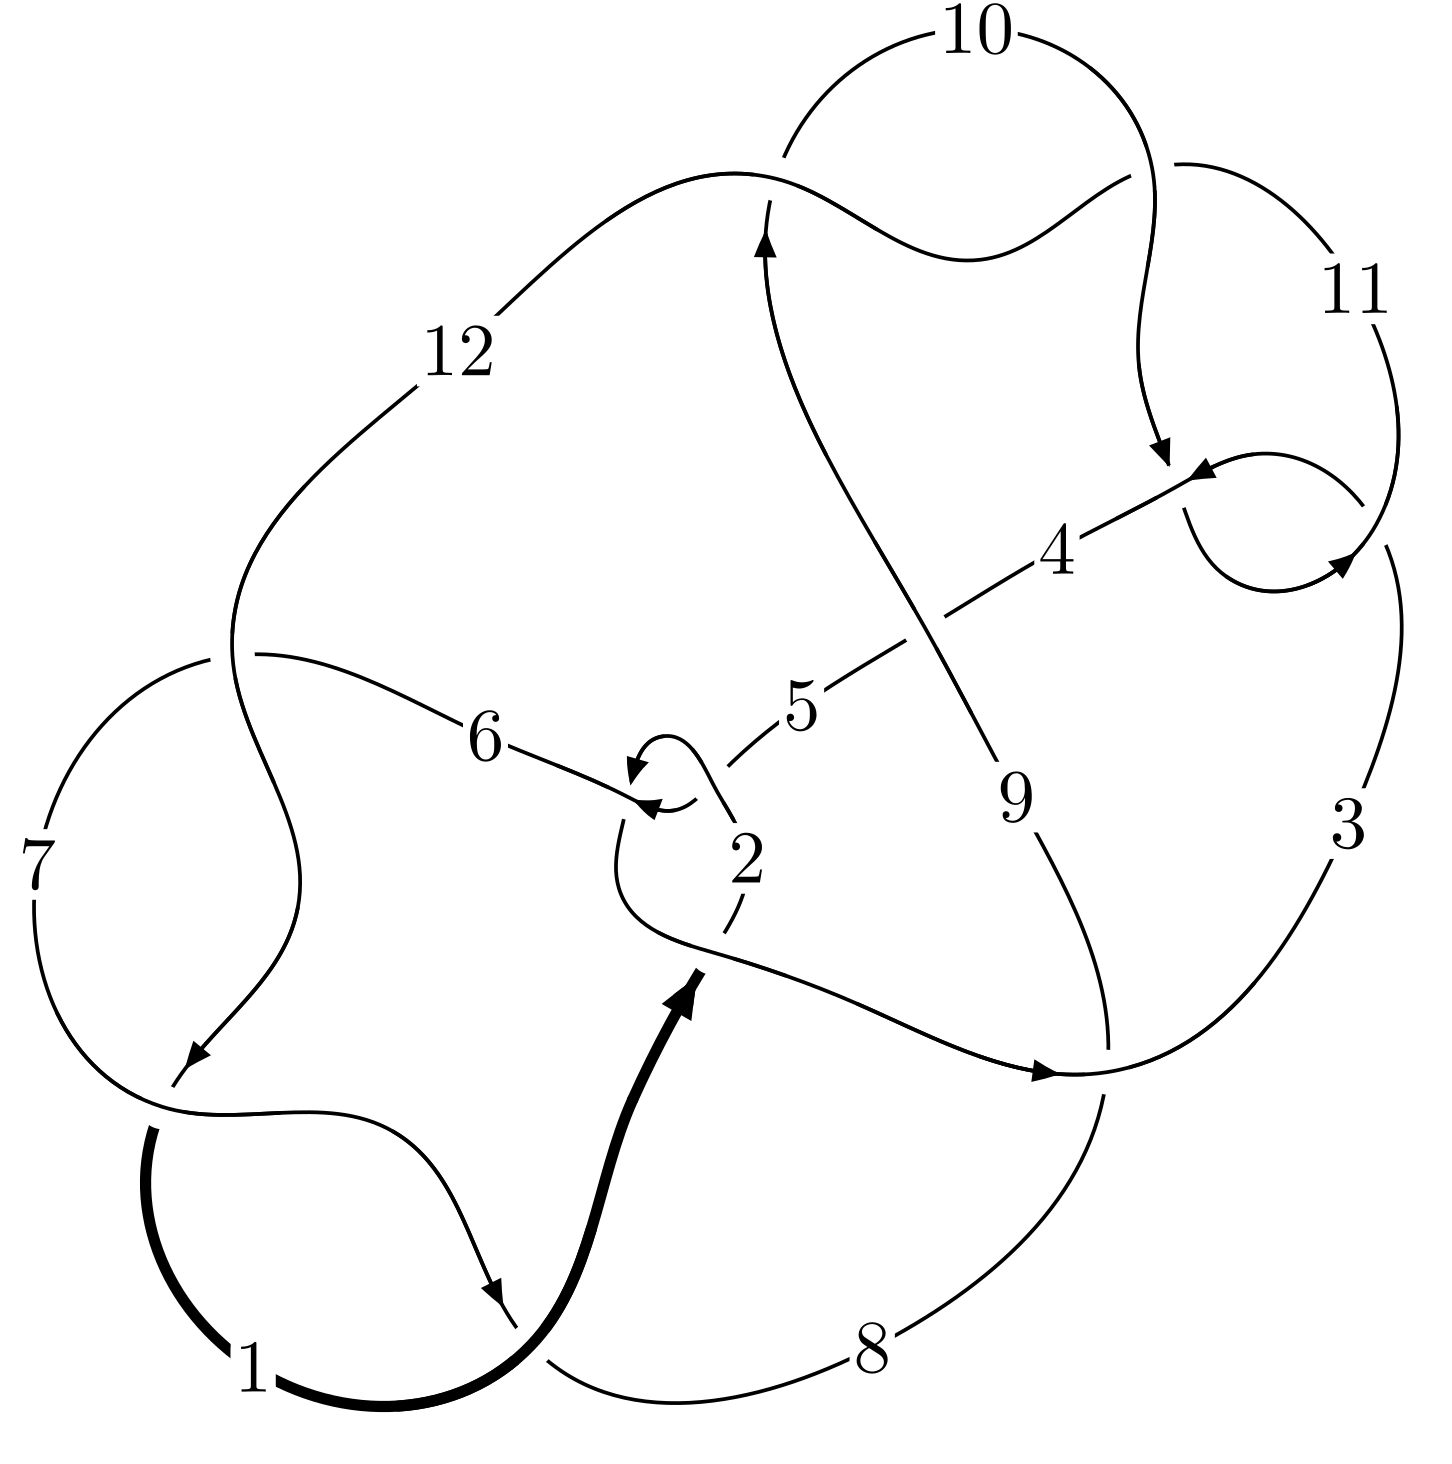
\includegraphics[width=112pt]{../../../GIT/diagram.site/Diagrams/png/2477_12n_0388.png}\\
\ \ \ A knot diagram\footnotemark}&
\allowdisplaybreaks
\textbf{Linearized knot diagam} \\
\cline{2-2}
 &
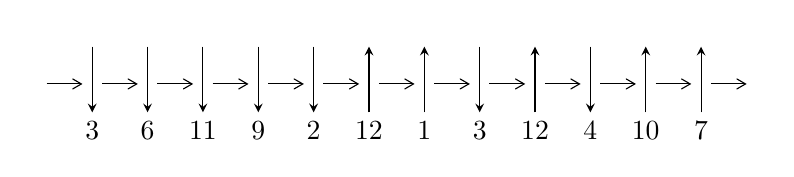
\begin{tikzpicture}[x=20pt, y=17pt]
	% nodes
	\node (C0) at (0, 0) {};
	\node (C1) at (1, 0) {};
	\node (C1U) at (1, +1) {};
	\node (C1D) at (1, -1) {3};

	\node (C2) at (2, 0) {};
	\node (C2U) at (2, +1) {};
	\node (C2D) at (2, -1) {6};

	\node (C3) at (3, 0) {};
	\node (C3U) at (3, +1) {};
	\node (C3D) at (3, -1) {11};

	\node (C4) at (4, 0) {};
	\node (C4U) at (4, +1) {};
	\node (C4D) at (4, -1) {9};

	\node (C5) at (5, 0) {};
	\node (C5U) at (5, +1) {};
	\node (C5D) at (5, -1) {2};

	\node (C6) at (6, 0) {};
	\node (C6U) at (6, +1) {};
	\node (C6D) at (6, -1) {12};

	\node (C7) at (7, 0) {};
	\node (C7U) at (7, +1) {};
	\node (C7D) at (7, -1) {1};

	\node (C8) at (8, 0) {};
	\node (C8U) at (8, +1) {};
	\node (C8D) at (8, -1) {3};

	\node (C9) at (9, 0) {};
	\node (C9U) at (9, +1) {};
	\node (C9D) at (9, -1) {12};

	\node (C10) at (10, 0) {};
	\node (C10U) at (10, +1) {};
	\node (C10D) at (10, -1) {4};

	\node (C11) at (11, 0) {};
	\node (C11U) at (11, +1) {};
	\node (C11D) at (11, -1) {10};

	\node (C12) at (12, 0) {};
	\node (C12U) at (12, +1) {};
	\node (C12D) at (12, -1) {7};
	\node (C13) at (13, 0) {};

	% arrows
	\draw[->,>={angle 60}]
	(C0) edge (C1) (C1) edge (C2) (C2) edge (C3) (C3) edge (C4) (C4) edge (C5) (C5) edge (C6) (C6) edge (C7) (C7) edge (C8) (C8) edge (C9) (C9) edge (C10) (C10) edge (C11) (C11) edge (C12) (C12) edge (C13) ;	\draw[->,>=stealth]
	(C1U) edge (C1D) (C2U) edge (C2D) (C3U) edge (C3D) (C4U) edge (C4D) (C5U) edge (C5D) (C6D) edge (C6U) (C7D) edge (C7U) (C8U) edge (C8D) (C9D) edge (C9U) (C10U) edge (C10D) (C11D) edge (C11U) (C12D) edge (C12U) ;
	\end{tikzpicture} \\
\hhline{~~} \\& 
\textbf{Solving Sequence} \\ \cline{2-2} 
 &
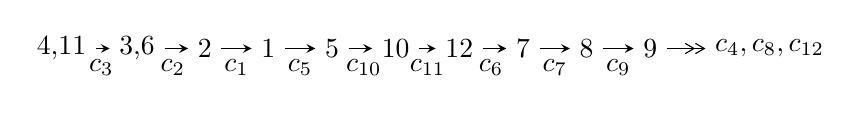
\begin{tikzpicture}[x=23pt, y=7pt]
	% node
	\node (A0) at (-1/8, 0) {4,11};
	\node (A1) at (17/16, 0) {3,6};
	\node (A2) at (17/8, 0) {2};
	\node (A3) at (25/8, 0) {1};
	\node (A4) at (33/8, 0) {5};
	\node (A5) at (41/8, 0) {10};
	\node (A6) at (49/8, 0) {12};
	\node (A7) at (57/8, 0) {7};
	\node (A8) at (65/8, 0) {8};
	\node (A9) at (73/8, 0) {9};
	\node (C1) at (1/2, -1) {$c_{3}$};
	\node (C2) at (13/8, -1) {$c_{2}$};
	\node (C3) at (21/8, -1) {$c_{1}$};
	\node (C4) at (29/8, -1) {$c_{5}$};
	\node (C5) at (37/8, -1) {$c_{10}$};
	\node (C6) at (45/8, -1) {$c_{11}$};
	\node (C7) at (53/8, -1) {$c_{6}$};
	\node (C8) at (61/8, -1) {$c_{7}$};
	\node (C9) at (69/8, -1) {$c_{9}$};
	\node (A10) at (11, 0) {$c_{4},c_{8},c_{12}$};

	% edge
	\draw[->,>=stealth]	
	(A0) edge (A1) (A1) edge (A2) (A2) edge (A3) (A3) edge (A4) (A4) edge (A5) (A5) edge (A6) (A6) edge (A7) (A7) edge (A8) (A8) edge (A9) ;
	\draw[->>,>={angle 60}]	
	(A9) edge (A10);
\end{tikzpicture} \\ 

\end{tabular} \\

\footnotetext{
The image of knot diagram is generated by the software ``\textbf{Draw programme}" developed by Andrew Bartholomew(\url{http://www.layer8.co.uk/maths/draw/index.htm\#Running-draw}), where we modified some parts for our purpose(\url{https://github.com/CATsTAILs/LinksPainter}).
}\phantom \\ \newline 
\centering \textbf{Ideals for irreducible components\footnotemark of $X_{\text{par}}$} 
 
\begin{align*}
I^u_{1}&=\langle 
- u^{25}+u^{24}+\cdots+4 b-4,\;-2 u^{26}+3 u^{25}+\cdots+4 a-2,\;u^{27}-2 u^{26}+\cdots-2 u^2+2\rangle \\
I^u_{2}&=\langle 
- u^2+b- u-1,\;- u^3-2 u^2+2 a- u,\;u^4+u^2+2\rangle \\
I^u_{3}&=\langle 
- a^2 u- a^2- a u+b+a-2,\;a^3+2 a^2 u-3 a u+u,\;u^2+u+1\rangle \\
I^u_{4}&=\langle 
b+u,\;a+u-1,\;u^2+1\rangle \\
I^u_{5}&=\langle 
u^3+u^2+b-1,\;a- u-1,\;u^4+1\rangle \\
\\
I^v_{1}&=\langle 
a,\;b-1,\;v-1\rangle \\
\end{align*}
\raggedright * 6 irreducible components of $\dim_{\mathbb{C}}=0$, with total 44 representations.\\
\footnotetext{All coefficients of polynomials are rational numbers. But the coefficients are sometimes approximated in decimal forms when there is not enough margin.}
\newpage
\renewcommand{\arraystretch}{1}
\centering \section*{I. $I^u_{1}= \langle - u^{25}+u^{24}+\cdots+4 b-4,\;-2 u^{26}+3 u^{25}+\cdots+4 a-2,\;u^{27}-2 u^{26}+\cdots-2 u^2+2 \rangle$}
\flushleft \textbf{(i) Arc colorings}\\
\begin{tabular}{m{7pt} m{180pt} m{7pt} m{180pt} }
\flushright $a_{4}=$&$\begin{pmatrix}1\\0\end{pmatrix}$ \\
\flushright $a_{11}=$&$\begin{pmatrix}0\\u\end{pmatrix}$ \\
\flushright $a_{3}=$&$\begin{pmatrix}1\\- u^2\end{pmatrix}$ \\
\flushright $a_{6}=$&$\begin{pmatrix}\frac{1}{2} u^{26}-\frac{3}{4} u^{25}+\cdots-\frac{1}{2} u+\frac{1}{2}\\\frac{1}{4} u^{25}-\frac{1}{4} u^{24}+\cdots+\frac{1}{2} u+1\end{pmatrix}$ \\
\flushright $a_{2}=$&$\begin{pmatrix}-\frac{1}{4} u^{22}- u^{20}+\cdots-\frac{1}{2} u+\frac{1}{2}\\\frac{1}{2} u^{17}+\frac{3}{2} u^{15}+\cdots- u^2+u\end{pmatrix}$ \\
\flushright $a_{1}=$&$\begin{pmatrix}-\frac{1}{4} u^{24}-\frac{5}{4} u^{22}+\cdots+\frac{1}{2} u+\frac{1}{2}\\\frac{1}{4} u^{26}+u^{24}+\cdots- u^2+u\end{pmatrix}$ \\
\flushright $a_{5}=$&$\begin{pmatrix}u^{10}+u^8+2 u^6+u^4+u^2+1\\u^{10}+2 u^8+3 u^6+2 u^4+u^2\end{pmatrix}$ \\
\flushright $a_{10}=$&$\begin{pmatrix}u\\u\end{pmatrix}$ \\
\flushright $a_{12}=$&$\begin{pmatrix}u^3\\u^3+u\end{pmatrix}$ \\
\flushright $a_{7}=$&$\begin{pmatrix}-\frac{1}{4} u^{22}- u^{20}+\cdots-\frac{3}{2} u+\frac{1}{2}\\\frac{1}{4} u^{24}+u^{22}+\cdots+\frac{1}{2} u^2- u\end{pmatrix}$ \\
\flushright $a_{8}=$&$\begin{pmatrix}- u^7-2 u^5-2 u^3-2 u\\u^9+u^7+u^5- u\end{pmatrix}$ \\
\flushright $a_{9}=$&$\begin{pmatrix}u^5+u\\u^5+u^3+u\end{pmatrix}$\\&\end{tabular}
\flushleft \textbf{(ii) Obstruction class $= -1$}\\~\\
\flushleft \textbf{(iii) Cusp Shapes $= 2 u^{26}-4 u^{25}+10 u^{24}-16 u^{23}+28 u^{22}-46 u^{21}+58 u^{20}-88 u^{19}+86 u^{18}-130 u^{17}+114 u^{16}-168 u^{15}+124 u^{14}-168 u^{13}+116 u^{12}-166 u^{11}+96 u^{10}-118 u^9+40 u^8-68 u^7+20 u^6-44 u^5-6 u^4+8 u^3-20 u^2+2 u-8$}\\~\\
\newpage\renewcommand{\arraystretch}{1}
\flushleft \textbf{(iv) u-Polynomials at the component}\newline \\
\begin{tabular}{m{50pt}|m{274pt}}
Crossings & \hspace{64pt}u-Polynomials at each crossing \\
\hline $$\begin{aligned}c_{1}\end{aligned}$$&$\begin{aligned}
&u^{27}-2 u^{26}+\cdots-1367 u+256
\end{aligned}$\\
\hline $$\begin{aligned}c_{2},c_{5}\end{aligned}$$&$\begin{aligned}
&u^{27}+2 u^{26}+\cdots-13 u+16
\end{aligned}$\\
\hline $$\begin{aligned}c_{3},c_{10}\end{aligned}$$&$\begin{aligned}
&u^{27}-2 u^{26}+\cdots-2 u^2+2
\end{aligned}$\\
\hline $$\begin{aligned}c_{4}\end{aligned}$$&$\begin{aligned}
&u^{27}-5 u^{26}+\cdots+4404 u+1706
\end{aligned}$\\
\hline $$\begin{aligned}c_{6},c_{7},c_{12}\end{aligned}$$&$\begin{aligned}
&u^{27}-2 u^{26}+\cdots+19 u+16
\end{aligned}$\\
\hline $$\begin{aligned}c_{8}\end{aligned}$$&$\begin{aligned}
&u^{27}+4 u^{26}+\cdots-358556 u+54322
\end{aligned}$\\
\hline $$\begin{aligned}c_{9},c_{11}\end{aligned}$$&$\begin{aligned}
&u^{27}-10 u^{26}+\cdots+8 u+4
\end{aligned}$\\
\hline
\end{tabular}\\~\\
\newpage\renewcommand{\arraystretch}{1}
\flushleft \textbf{(v) Riley Polynomials at the component}\newline \\
\begin{tabular}{m{50pt}|m{274pt}}
Crossings & \hspace{64pt}Riley Polynomials at each crossing \\
\hline $$\begin{aligned}c_{1}\end{aligned}$$&$\begin{aligned}
&y^{27}+74 y^{26}+\cdots+1160081 y-65536
\end{aligned}$\\
\hline $$\begin{aligned}c_{2},c_{5}\end{aligned}$$&$\begin{aligned}
&y^{27}+2 y^{26}+\cdots-1367 y-256
\end{aligned}$\\
\hline $$\begin{aligned}c_{3},c_{10}\end{aligned}$$&$\begin{aligned}
&y^{27}+10 y^{26}+\cdots+8 y-4
\end{aligned}$\\
\hline $$\begin{aligned}c_{4}\end{aligned}$$&$\begin{aligned}
&y^{27}+49 y^{26}+\cdots-17215544 y-2910436
\end{aligned}$\\
\hline $$\begin{aligned}c_{6},c_{7},c_{12}\end{aligned}$$&$\begin{aligned}
&y^{27}-46 y^{26}+\cdots-2839 y-256
\end{aligned}$\\
\hline $$\begin{aligned}c_{8}\end{aligned}$$&$\begin{aligned}
&y^{27}+82 y^{26}+\cdots+70277723880 y-2950879684
\end{aligned}$\\
\hline $$\begin{aligned}c_{9},c_{11}\end{aligned}$$&$\begin{aligned}
&y^{27}+14 y^{26}+\cdots+1024 y-16
\end{aligned}$\\
\hline
\end{tabular}\\~\\
\newpage\flushleft \textbf{(vi) Complex Volumes and Cusp Shapes}
$$\begin{array}{c|c|c}  
\text{Solutions to }I^u_{1}& \I (\text{vol} + \sqrt{-1}CS) & \text{Cusp shape}\\
 \hline 
\begin{aligned}
u &= \phantom{-}0.697654 + 0.748808 I \\
a &= \phantom{-}1.026780 + 0.002420 I \\
b &= \phantom{-}1.06126 - 1.23166 I\end{aligned}
 & -3.52813 + 0.07338 I & -9.79527 - 0.84081 I \\ \hline\begin{aligned}
u &= \phantom{-}0.697654 - 0.748808 I \\
a &= \phantom{-}1.026780 - 0.002420 I \\
b &= \phantom{-}1.06126 + 1.23166 I\end{aligned}
 & -3.52813 - 0.07338 I & -9.79527 + 0.84081 I \\ \hline\begin{aligned}
u &= \phantom{-}0.864921 + 0.447342 I \\
a &= -0.587169 + 0.347747 I \\
b &= -0.479795 - 0.989527 I\end{aligned}
 & \phantom{-}12.22120 - 2.26521 I & -0.78342 + 1.87468 I \\ \hline\begin{aligned}
u &= \phantom{-}0.864921 - 0.447342 I \\
a &= -0.587169 - 0.347747 I \\
b &= -0.479795 + 0.989527 I\end{aligned}
 & \phantom{-}12.22120 + 2.26521 I & -0.78342 - 1.87468 I \\ \hline\begin{aligned}
u &= -0.770627 + 0.681378 I \\
a &= \phantom{-}0.728531 - 0.074268 I \\
b &= \phantom{-}0.086141 + 1.355080 I\end{aligned}
 & \phantom{-}0.458304 - 0.114158 I & \phantom{-}0.422197 - 0.454382 I \\ \hline\begin{aligned}
u &= -0.770627 - 0.681378 I \\
a &= \phantom{-}0.728531 + 0.074268 I \\
b &= \phantom{-}0.086141 - 1.355080 I\end{aligned}
 & \phantom{-}0.458304 + 0.114158 I & \phantom{-}0.422197 + 0.454382 I \\ \hline\begin{aligned}
u &= -0.878083 + 0.542301 I \\
a &= -0.606653 + 0.267104 I \\
b &= -1.19080 - 1.81606 I\end{aligned}
 & \phantom{-}11.64340 - 6.38697 I & -1.19981 + 2.11434 I \\ \hline\begin{aligned}
u &= -0.878083 - 0.542301 I \\
a &= -0.606653 - 0.267104 I \\
b &= -1.19080 + 1.81606 I\end{aligned}
 & \phantom{-}11.64340 + 6.38697 I & -1.19981 - 2.11434 I \\ \hline\begin{aligned}
u &= \phantom{-}0.100635 + 1.097690 I \\
a &= -0.85192 + 1.71040 I \\
b &= -0.550049 + 1.253330 I\end{aligned}
 & \phantom{-}6.60434 + 0.15878 I & \phantom{-}5.87983 + 0.02677 I \\ \hline\begin{aligned}
u &= \phantom{-}0.100635 - 1.097690 I \\
a &= -0.85192 - 1.71040 I \\
b &= -0.550049 - 1.253330 I\end{aligned}
 & \phantom{-}6.60434 - 0.15878 I & \phantom{-}5.87983 - 0.02677 I\\
 \hline 
 \end{array}$$\newpage$$\begin{array}{c|c|c}  
\text{Solutions to }I^u_{1}& \I (\text{vol} + \sqrt{-1}CS) & \text{Cusp shape}\\
 \hline 
\begin{aligned}
u &= \phantom{-}0.669390 + 0.942059 I \\
a &= -0.88412 + 1.56066 I \\
b &= \phantom{-}0.57563 + 1.56765 I\end{aligned}
 & -2.93763 - 5.34360 I & -7.41989 + 6.92820 I \\ \hline\begin{aligned}
u &= \phantom{-}0.669390 - 0.942059 I \\
a &= -0.88412 - 1.56066 I \\
b &= \phantom{-}0.57563 - 1.56765 I\end{aligned}
 & -2.93763 + 5.34360 I & -7.41989 - 6.92820 I \\ \hline\begin{aligned}
u &= \phantom{-}0.686168 + 0.447957 I \\
a &= \phantom{-}0.405997 - 0.432049 I \\
b &= -0.812403 + 0.706687 I\end{aligned}
 & \phantom{-}1.78018 + 2.00372 I & -0.59189 - 2.09997 I \\ \hline\begin{aligned}
u &= \phantom{-}0.686168 - 0.447957 I \\
a &= \phantom{-}0.405997 + 0.432049 I \\
b &= -0.812403 - 0.706687 I\end{aligned}
 & \phantom{-}1.78018 - 2.00372 I & -0.59189 + 2.09997 I \\ \hline\begin{aligned}
u &= \phantom{-}0.040008 + 1.207920 I \\
a &= -0.99416 - 2.11968 I \\
b &= -0.43164 - 1.73930 I\end{aligned}
 & \phantom{-}18.1739 - 4.5997 I & \phantom{-}4.36505 + 2.18290 I \\ \hline\begin{aligned}
u &= \phantom{-}0.040008 - 1.207920 I \\
a &= -0.99416 + 2.11968 I \\
b &= -0.43164 + 1.73930 I\end{aligned}
 & \phantom{-}18.1739 + 4.5997 I & \phantom{-}4.36505 - 2.18290 I \\ \hline\begin{aligned}
u &= \phantom{-}0.601091 + 1.054470 I \\
a &= \phantom{-}0.61079 - 1.66086 I \\
b &= -1.15984 - 0.98023 I\end{aligned}
 & \phantom{-}3.48901 - 6.97695 I & \phantom{-}1.70016 + 6.49908 I \\ \hline\begin{aligned}
u &= \phantom{-}0.601091 - 1.054470 I \\
a &= \phantom{-}0.61079 + 1.66086 I \\
b &= -1.15984 + 0.98023 I\end{aligned}
 & \phantom{-}3.48901 + 6.97695 I & \phantom{-}1.70016 - 6.49908 I \\ \hline\begin{aligned}
u &= -0.710977 + 1.000460 I \\
a &= -1.42612 - 0.55763 I \\
b &= -0.14675 - 1.63948 I\end{aligned}
 & \phantom{-}1.40487 + 5.73270 I & \phantom{-}1.73930 - 4.91111 I \\ \hline\begin{aligned}
u &= -0.710977 - 1.000460 I \\
a &= -1.42612 + 0.55763 I \\
b &= -0.14675 + 1.63948 I\end{aligned}
 & \phantom{-}1.40487 - 5.73270 I & \phantom{-}1.73930 + 4.91111 I\\
 \hline 
 \end{array}$$\newpage$$\begin{array}{c|c|c}  
\text{Solutions to }I^u_{1}& \I (\text{vol} + \sqrt{-1}CS) & \text{Cusp shape}\\
 \hline 
\begin{aligned}
u &= -0.074391 + 0.718228 I \\
a &= \phantom{-}0.98792 - 1.24993 I \\
b &= -0.006103 - 0.217922 I\end{aligned}
 & \phantom{-}0.94642 + 1.42613 I & \phantom{-}1.85713 - 5.82586 I \\ \hline\begin{aligned}
u &= -0.074391 - 0.718228 I \\
a &= \phantom{-}0.98792 + 1.24993 I \\
b &= -0.006103 + 0.217922 I\end{aligned}
 & \phantom{-}0.94642 - 1.42613 I & \phantom{-}1.85713 + 5.82586 I \\ \hline\begin{aligned}
u &= \phantom{-}0.638164 + 1.116710 I \\
a &= -1.48999 + 0.10418 I \\
b &= -0.054880 + 0.864766 I\end{aligned}
 & \phantom{-}14.2506 - 3.2919 I & \phantom{-}1.72901 + 2.48936 I \\ \hline\begin{aligned}
u &= \phantom{-}0.638164 - 1.116710 I \\
a &= -1.48999 - 0.10418 I \\
b &= -0.054880 - 0.864766 I\end{aligned}
 & \phantom{-}14.2506 + 3.2919 I & \phantom{-}1.72901 - 2.48936 I \\ \hline\begin{aligned}
u &= -0.688671 + 1.094800 I \\
a &= \phantom{-}1.11378 + 2.20355 I \\
b &= -1.22699 + 2.17626 I\end{aligned}
 & \phantom{-}13.3230 + 12.1918 I & \phantom{-}0.72580 - 6.39342 I \\ \hline\begin{aligned}
u &= -0.688671 - 1.094800 I \\
a &= \phantom{-}1.11378 - 2.20355 I \\
b &= -1.22699 - 2.17626 I\end{aligned}
 & \phantom{-}13.3230 - 12.1918 I & \phantom{-}0.72580 + 6.39342 I \\ \hline\begin{aligned}
u &= -0.350564\phantom{ +0.000000I} \\
a &= \phantom{-}0.932661\phantom{ +0.000000I} \\
b &= \phantom{-}0.672452\phantom{ +0.000000I}\end{aligned}
 & -1.03514\phantom{ +0.000000I} & -11.2560\phantom{ +0.000000I}\\
 \hline 
 \end{array}$$\newpage\newpage\renewcommand{\arraystretch}{1}
\centering \section*{II. $I^u_{2}= \langle - u^2+b- u-1,\;- u^3-2 u^2+2 a- u,\;u^4+u^2+2 \rangle$}
\flushleft \textbf{(i) Arc colorings}\\
\begin{tabular}{m{7pt} m{180pt} m{7pt} m{180pt} }
\flushright $a_{4}=$&$\begin{pmatrix}1\\0\end{pmatrix}$ \\
\flushright $a_{11}=$&$\begin{pmatrix}0\\u\end{pmatrix}$ \\
\flushright $a_{3}=$&$\begin{pmatrix}1\\- u^2\end{pmatrix}$ \\
\flushright $a_{6}=$&$\begin{pmatrix}\frac{1}{2} u^3+u^2+\frac{1}{2} u\\u^2+u+1\end{pmatrix}$ \\
\flushright $a_{2}=$&$\begin{pmatrix}\frac{1}{2} u^3+u^2+\frac{1}{2} u+1\\u+1\end{pmatrix}$ \\
\flushright $a_{1}=$&$\begin{pmatrix}\frac{1}{2} u^3+u^2+\frac{1}{2} u\\u^2+u+1\end{pmatrix}$ \\
\flushright $a_{5}=$&$\begin{pmatrix}-1\\u^2\end{pmatrix}$ \\
\flushright $a_{10}=$&$\begin{pmatrix}u\\u\end{pmatrix}$ \\
\flushright $a_{12}=$&$\begin{pmatrix}u^3\\u^3+u\end{pmatrix}$ \\
\flushright $a_{7}=$&$\begin{pmatrix}-\frac{1}{2} u^3+u^2+\frac{1}{2} u\\- u^3+u^2+1\end{pmatrix}$ \\
\flushright $a_{8}=$&$\begin{pmatrix}- u^3\\- u^3- u\end{pmatrix}$ \\
\flushright $a_{9}=$&$\begin{pmatrix}- u^3- u\\- u\end{pmatrix}$\\&\end{tabular}
\flushleft \textbf{(ii) Obstruction class $= 1$}\\~\\
\flushleft \textbf{(iii) Cusp Shapes $= 4 u^2$}\\~\\
\newpage\renewcommand{\arraystretch}{1}
\flushleft \textbf{(iv) u-Polynomials at the component}\newline \\
\begin{tabular}{m{50pt}|m{274pt}}
Crossings & \hspace{64pt}u-Polynomials at each crossing \\
\hline $$\begin{aligned}c_{1},c_{5},c_{6}\\c_{7}\end{aligned}$$&$\begin{aligned}
&(u-1)^4
\end{aligned}$\\
\hline $$\begin{aligned}c_{2},c_{12}\end{aligned}$$&$\begin{aligned}
&(u+1)^4
\end{aligned}$\\
\hline $$\begin{aligned}c_{3},c_{4},c_{8}\\c_{10}\end{aligned}$$&$\begin{aligned}
&u^4+u^2+2
\end{aligned}$\\
\hline $$\begin{aligned}c_{9}\end{aligned}$$&$\begin{aligned}
&(u^2+u+2)^2
\end{aligned}$\\
\hline $$\begin{aligned}c_{11}\end{aligned}$$&$\begin{aligned}
&(u^2- u+2)^2
\end{aligned}$\\
\hline
\end{tabular}\\~\\
\newpage\renewcommand{\arraystretch}{1}
\flushleft \textbf{(v) Riley Polynomials at the component}\newline \\
\begin{tabular}{m{50pt}|m{274pt}}
Crossings & \hspace{64pt}Riley Polynomials at each crossing \\
\hline $$\begin{aligned}c_{1},c_{2},c_{5}\\c_{6},c_{7},c_{12}\end{aligned}$$&$\begin{aligned}
&(y-1)^4
\end{aligned}$\\
\hline $$\begin{aligned}c_{3},c_{4},c_{8}\\c_{10}\end{aligned}$$&$\begin{aligned}
&(y^2+y+2)^2
\end{aligned}$\\
\hline $$\begin{aligned}c_{9},c_{11}\end{aligned}$$&$\begin{aligned}
&(y^2+3 y+4)^2
\end{aligned}$\\
\hline
\end{tabular}\\~\\
\newpage\flushleft \textbf{(vi) Complex Volumes and Cusp Shapes}
$$\begin{array}{c|c|c}  
\text{Solutions to }I^u_{2}& \I (\text{vol} + \sqrt{-1}CS) & \text{Cusp shape}\\
 \hline 
\begin{aligned}
u &= \phantom{-}0.676097 + 0.978318 I \\
a &= -0.97807 + 2.01465 I \\
b &= \phantom{-}1.17610 + 2.30119 I\end{aligned}
 & -0.82247 - 5.33349 I & -2.00000 + 5.29150 I \\ \hline\begin{aligned}
u &= \phantom{-}0.676097 - 0.978318 I \\
a &= -0.97807 - 2.01465 I \\
b &= \phantom{-}1.17610 - 2.30119 I\end{aligned}
 & -0.82247 + 5.33349 I & -2.00000 - 5.29150 I \\ \hline\begin{aligned}
u &= -0.676097 + 0.978318 I \\
a &= -0.021927 - 0.631100 I \\
b &= -0.176097 - 0.344557 I\end{aligned}
 & -0.82247 + 5.33349 I & -2.00000 - 5.29150 I \\ \hline\begin{aligned}
u &= -0.676097 - 0.978318 I \\
a &= -0.021927 + 0.631100 I \\
b &= -0.176097 + 0.344557 I\end{aligned}
 & -0.82247 - 5.33349 I & -2.00000 + 5.29150 I\\
 \hline 
 \end{array}$$\newpage\newpage\renewcommand{\arraystretch}{1}
\centering \section*{III. $I^u_{3}= \langle - a^2 u- a^2- a u+b+a-2,\;a^3+2 a^2 u-3 a u+u,\;u^2+u+1 \rangle$}
\flushleft \textbf{(i) Arc colorings}\\
\begin{tabular}{m{7pt} m{180pt} m{7pt} m{180pt} }
\flushright $a_{4}=$&$\begin{pmatrix}1\\0\end{pmatrix}$ \\
\flushright $a_{11}=$&$\begin{pmatrix}0\\u\end{pmatrix}$ \\
\flushright $a_{3}=$&$\begin{pmatrix}1\\u+1\end{pmatrix}$ \\
\flushright $a_{6}=$&$\begin{pmatrix}a\\a^2 u+a^2+a u- a+2\end{pmatrix}$ \\
\flushright $a_{2}=$&$\begin{pmatrix}a\\- a^2 u- a^2+2 a-2\end{pmatrix}$ \\
\flushright $a_{1}=$&$\begin{pmatrix}- a^2 u- a^2- a u+2 a-2\\-2 a^2 u- a^2+a u+4 a-2 u-4\end{pmatrix}$ \\
\flushright $a_{5}=$&$\begin{pmatrix}1\\0\end{pmatrix}$ \\
\flushright $a_{10}=$&$\begin{pmatrix}u\\u\end{pmatrix}$ \\
\flushright $a_{12}=$&$\begin{pmatrix}1\\u+1\end{pmatrix}$ \\
\flushright $a_{7}=$&$\begin{pmatrix}a^2 u+a^2- a+2\\2 a^2 u+a^2- a u-3 a+2 u+4\end{pmatrix}$ \\
\flushright $a_{8}=$&$\begin{pmatrix}- u\\- u\end{pmatrix}$ \\
\flushright $a_{9}=$&$\begin{pmatrix}-1\\0\end{pmatrix}$\\&\end{tabular}
\flushleft \textbf{(ii) Obstruction class $= -1$}\\~\\
\flushleft \textbf{(iii) Cusp Shapes $= -4 u-2$}\\~\\
\newpage\renewcommand{\arraystretch}{1}
\flushleft \textbf{(iv) u-Polynomials at the component}\newline \\
\begin{tabular}{m{50pt}|m{274pt}}
Crossings & \hspace{64pt}u-Polynomials at each crossing \\
\hline $$\begin{aligned}c_{1}\end{aligned}$$&$\begin{aligned}
&u^6+4 u^5+6 u^4+3 u^3- u^2- u+1
\end{aligned}$\\
\hline $$\begin{aligned}c_{2},c_{5},c_{6}\\c_{7},c_{12}\end{aligned}$$&$\begin{aligned}
&u^6-2 u^4+u^3+u^2- u+1
\end{aligned}$\\
\hline $$\begin{aligned}c_{3},c_{10}\end{aligned}$$&$\begin{aligned}
&(u^2+u+1)^3
\end{aligned}$\\
\hline $$\begin{aligned}c_{4}\end{aligned}$$&$\begin{aligned}
&u^6
\end{aligned}$\\
\hline $$\begin{aligned}c_{8},c_{9},c_{11}\end{aligned}$$&$\begin{aligned}
&(u^2- u+1)^3
\end{aligned}$\\
\hline
\end{tabular}\\~\\
\newpage\renewcommand{\arraystretch}{1}
\flushleft \textbf{(v) Riley Polynomials at the component}\newline \\
\begin{tabular}{m{50pt}|m{274pt}}
Crossings & \hspace{64pt}Riley Polynomials at each crossing \\
\hline $$\begin{aligned}c_{1}\end{aligned}$$&$\begin{aligned}
&y^6-4 y^5+10 y^4-11 y^3+19 y^2-3 y+1
\end{aligned}$\\
\hline $$\begin{aligned}c_{2},c_{5},c_{6}\\c_{7},c_{12}\end{aligned}$$&$\begin{aligned}
&y^6-4 y^5+6 y^4-3 y^3- y^2+y+1
\end{aligned}$\\
\hline $$\begin{aligned}c_{3},c_{8},c_{9}\\c_{10},c_{11}\end{aligned}$$&$\begin{aligned}
&(y^2+y+1)^3
\end{aligned}$\\
\hline $$\begin{aligned}c_{4}\end{aligned}$$&$\begin{aligned}
&y^6
\end{aligned}$\\
\hline
\end{tabular}\\~\\
\newpage\flushleft \textbf{(vi) Complex Volumes and Cusp Shapes}
$$\begin{array}{c|c|c}  
\text{Solutions to }I^u_{3}& \I (\text{vol} + \sqrt{-1}CS) & \text{Cusp shape}\\
 \hline 
\begin{aligned}
u &= -0.500000 + 0.866025 I \\
a &= \phantom{-}0.741145 + 0.632163 I \\
b &= -0.395862 + 0.291743 I\end{aligned}
 & \phantom{-0.000000 -}2.02988 I & \phantom{-0.000000 } 0. - 3.46410 I \\ \hline\begin{aligned}
u &= -0.500000 + 0.866025 I \\
a &= \phantom{-}0.439111 - 0.046276 I \\
b &= \phantom{-}1.51194 + 0.59451 I\end{aligned}
 & \phantom{-0.000000 -}2.02988 I & \phantom{-0.000000 } 0. - 3.46410 I \\ \hline\begin{aligned}
u &= -0.500000 + 0.866025 I \\
a &= -0.18026 - 2.31794 I \\
b &= \phantom{-}0.883917 - 0.886250 I\end{aligned}
 & \phantom{-0.000000 -}2.02988 I & \phantom{-0.000000 } 0. - 3.46410 I \\ \hline\begin{aligned}
u &= -0.500000 - 0.866025 I \\
a &= \phantom{-}0.741145 - 0.632163 I \\
b &= -0.395862 - 0.291743 I\end{aligned}
 & \phantom{-0.000000 } -2.02988 I & \phantom{-0.000000 -}0. + 3.46410 I \\ \hline\begin{aligned}
u &= -0.500000 - 0.866025 I \\
a &= \phantom{-}0.439111 + 0.046276 I \\
b &= \phantom{-}1.51194 - 0.59451 I\end{aligned}
 & \phantom{-0.000000 } -2.02988 I & \phantom{-0.000000 -}0. + 3.46410 I \\ \hline\begin{aligned}
u &= -0.500000 - 0.866025 I \\
a &= -0.18026 + 2.31794 I \\
b &= \phantom{-}0.883917 + 0.886250 I\end{aligned}
 & \phantom{-0.000000 } -2.02988 I & \phantom{-0.000000 -}0. + 3.46410 I\\
 \hline 
 \end{array}$$\newpage\newpage\renewcommand{\arraystretch}{1}
\centering \section*{IV. $I^u_{4}= \langle b+u,\;a+u-1,\;u^2+1 \rangle$}
\flushleft \textbf{(i) Arc colorings}\\
\begin{tabular}{m{7pt} m{180pt} m{7pt} m{180pt} }
\flushright $a_{4}=$&$\begin{pmatrix}1\\0\end{pmatrix}$ \\
\flushright $a_{11}=$&$\begin{pmatrix}0\\u\end{pmatrix}$ \\
\flushright $a_{3}=$&$\begin{pmatrix}1\\1\end{pmatrix}$ \\
\flushright $a_{6}=$&$\begin{pmatrix}- u+1\\- u\end{pmatrix}$ \\
\flushright $a_{2}=$&$\begin{pmatrix}- u+2\\- u+1\end{pmatrix}$ \\
\flushright $a_{1}=$&$\begin{pmatrix}- u+1\\- u\end{pmatrix}$ \\
\flushright $a_{5}=$&$\begin{pmatrix}-1\\-1\end{pmatrix}$ \\
\flushright $a_{10}=$&$\begin{pmatrix}u\\u\end{pmatrix}$ \\
\flushright $a_{12}=$&$\begin{pmatrix}- u\\0\end{pmatrix}$ \\
\flushright $a_{7}=$&$\begin{pmatrix}1\\- u\end{pmatrix}$ \\
\flushright $a_{8}=$&$\begin{pmatrix}u\\0\end{pmatrix}$ \\
\flushright $a_{9}=$&$\begin{pmatrix}2 u\\u\end{pmatrix}$\\&\end{tabular}
\flushleft \textbf{(ii) Obstruction class $= 1$}\\~\\
\flushleft \textbf{(iii) Cusp Shapes $= 4$}\\~\\
\newpage\renewcommand{\arraystretch}{1}
\flushleft \textbf{(iv) u-Polynomials at the component}\newline \\
\begin{tabular}{m{50pt}|m{274pt}}
Crossings & \hspace{64pt}u-Polynomials at each crossing \\
\hline $$\begin{aligned}c_{1},c_{5},c_{6}\\c_{7},c_{11}\end{aligned}$$&$\begin{aligned}
&(u-1)^2
\end{aligned}$\\
\hline $$\begin{aligned}c_{2},c_{9},c_{12}\end{aligned}$$&$\begin{aligned}
&(u+1)^2
\end{aligned}$\\
\hline $$\begin{aligned}c_{3},c_{4},c_{8}\\c_{10}\end{aligned}$$&$\begin{aligned}
&u^2+1
\end{aligned}$\\
\hline
\end{tabular}\\~\\
\newpage\renewcommand{\arraystretch}{1}
\flushleft \textbf{(v) Riley Polynomials at the component}\newline \\
\begin{tabular}{m{50pt}|m{274pt}}
Crossings & \hspace{64pt}Riley Polynomials at each crossing \\
\hline $$\begin{aligned}c_{1},c_{2},c_{5}\\c_{6},c_{7},c_{9}\\c_{11},c_{12}\end{aligned}$$&$\begin{aligned}
&(y-1)^2
\end{aligned}$\\
\hline $$\begin{aligned}c_{3},c_{4},c_{8}\\c_{10}\end{aligned}$$&$\begin{aligned}
&(y+1)^2
\end{aligned}$\\
\hline
\end{tabular}\\~\\
\newpage\flushleft \textbf{(vi) Complex Volumes and Cusp Shapes}
$$\begin{array}{c|c|c}  
\text{Solutions to }I^u_{4}& \I (\text{vol} + \sqrt{-1}CS) & \text{Cusp shape}\\
 \hline 
\begin{aligned}
u &= \phantom{-0.000000 -}1.000000 I \\
a &= \phantom{-}1.00000 - 1.00000 I \\
b &= \phantom{-0.000000 } -1.000000 I\end{aligned}
 & \phantom{-}3.28987\phantom{ +0.000000I} & \phantom{-}4.00000\phantom{ +0.000000I} \\ \hline\begin{aligned}
u &= \phantom{-0.000000 } -1.000000 I \\
a &= \phantom{-}1.00000 + 1.00000 I \\
b &= \phantom{-0.000000 -}1.000000 I\end{aligned}
 & \phantom{-}3.28987\phantom{ +0.000000I} & \phantom{-}4.00000\phantom{ +0.000000I}\\
 \hline 
 \end{array}$$\newpage\newpage\renewcommand{\arraystretch}{1}
\centering \section*{V. $I^u_{5}= \langle u^3+u^2+b-1,\;a- u-1,\;u^4+1 \rangle$}
\flushleft \textbf{(i) Arc colorings}\\
\begin{tabular}{m{7pt} m{180pt} m{7pt} m{180pt} }
\flushright $a_{4}=$&$\begin{pmatrix}1\\0\end{pmatrix}$ \\
\flushright $a_{11}=$&$\begin{pmatrix}0\\u\end{pmatrix}$ \\
\flushright $a_{3}=$&$\begin{pmatrix}1\\- u^2\end{pmatrix}$ \\
\flushright $a_{6}=$&$\begin{pmatrix}u+1\\- u^3- u^2+1\end{pmatrix}$ \\
\flushright $a_{2}=$&$\begin{pmatrix}- u\\u^3-1\end{pmatrix}$ \\
\flushright $a_{1}=$&$\begin{pmatrix}- u-1\\u^3+u^2-1\end{pmatrix}$ \\
\flushright $a_{5}=$&$\begin{pmatrix}1\\- u^2\end{pmatrix}$ \\
\flushright $a_{10}=$&$\begin{pmatrix}u\\u\end{pmatrix}$ \\
\flushright $a_{12}=$&$\begin{pmatrix}u^3\\u^3+u\end{pmatrix}$ \\
\flushright $a_{7}=$&$\begin{pmatrix}u^3+u+1\\- u^2+u+1\end{pmatrix}$ \\
\flushright $a_{8}=$&$\begin{pmatrix}u^3\\u^3+u\end{pmatrix}$ \\
\flushright $a_{9}=$&$\begin{pmatrix}0\\u^3\end{pmatrix}$\\&\end{tabular}
\flushleft \textbf{(ii) Obstruction class $= 1$}\\~\\
\flushleft \textbf{(iii) Cusp Shapes $= -4$}\\~\\
\newpage\renewcommand{\arraystretch}{1}
\flushleft \textbf{(iv) u-Polynomials at the component}\newline \\
\begin{tabular}{m{50pt}|m{274pt}}
Crossings & \hspace{64pt}u-Polynomials at each crossing \\
\hline $$\begin{aligned}c_{1},c_{2},c_{12}\end{aligned}$$&$\begin{aligned}
&(u-1)^4
\end{aligned}$\\
\hline $$\begin{aligned}c_{3},c_{4},c_{8}\\c_{10}\end{aligned}$$&$\begin{aligned}
&u^4+1
\end{aligned}$\\
\hline $$\begin{aligned}c_{5},c_{6},c_{7}\end{aligned}$$&$\begin{aligned}
&(u+1)^4
\end{aligned}$\\
\hline $$\begin{aligned}c_{9},c_{11}\end{aligned}$$&$\begin{aligned}
&(u^2+1)^2
\end{aligned}$\\
\hline
\end{tabular}\\~\\
\newpage\renewcommand{\arraystretch}{1}
\flushleft \textbf{(v) Riley Polynomials at the component}\newline \\
\begin{tabular}{m{50pt}|m{274pt}}
Crossings & \hspace{64pt}Riley Polynomials at each crossing \\
\hline $$\begin{aligned}c_{1},c_{2},c_{5}\\c_{6},c_{7},c_{12}\end{aligned}$$&$\begin{aligned}
&(y-1)^4
\end{aligned}$\\
\hline $$\begin{aligned}c_{3},c_{4},c_{8}\\c_{10}\end{aligned}$$&$\begin{aligned}
&(y^2+1)^2
\end{aligned}$\\
\hline $$\begin{aligned}c_{9},c_{11}\end{aligned}$$&$\begin{aligned}
&(y+1)^4
\end{aligned}$\\
\hline
\end{tabular}\\~\\
\newpage\flushleft \textbf{(vi) Complex Volumes and Cusp Shapes}
$$\begin{array}{c|c|c}  
\text{Solutions to }I^u_{5}& \I (\text{vol} + \sqrt{-1}CS) & \text{Cusp shape}\\
 \hline 
\begin{aligned}
u &= \phantom{-}0.707107 + 0.707107 I \\
a &= \phantom{-}1.70711 + 0.70711 I \\
b &= \phantom{-}1.70711 - 1.70711 I\end{aligned}
 & -1.64493\phantom{ +0.000000I} & -4.00000\phantom{ +0.000000I} \\ \hline\begin{aligned}
u &= \phantom{-}0.707107 - 0.707107 I \\
a &= \phantom{-}1.70711 - 0.70711 I \\
b &= \phantom{-}1.70711 + 1.70711 I\end{aligned}
 & -1.64493\phantom{ +0.000000I} & -4.00000\phantom{ +0.000000I} \\ \hline\begin{aligned}
u &= -0.707107 + 0.707107 I \\
a &= \phantom{-}0.292893 + 0.707107 I \\
b &= \phantom{-}0.292893 + 0.292893 I\end{aligned}
 & -1.64493\phantom{ +0.000000I} & -4.00000\phantom{ +0.000000I} \\ \hline\begin{aligned}
u &= -0.707107 - 0.707107 I \\
a &= \phantom{-}0.292893 - 0.707107 I \\
b &= \phantom{-}0.292893 - 0.292893 I\end{aligned}
 & -1.64493\phantom{ +0.000000I} & -4.00000\phantom{ +0.000000I}\\
 \hline 
 \end{array}$$\newpage\newpage\renewcommand{\arraystretch}{1}
\centering \section*{VI. $I^v_{1}= \langle a,\;b-1,\;v-1 \rangle$}
\flushleft \textbf{(i) Arc colorings}\\
\begin{tabular}{m{7pt} m{180pt} m{7pt} m{180pt} }
\flushright $a_{4}=$&$\begin{pmatrix}1\\0\end{pmatrix}$ \\
\flushright $a_{11}=$&$\begin{pmatrix}1\\0\end{pmatrix}$ \\
\flushright $a_{3}=$&$\begin{pmatrix}1\\0\end{pmatrix}$ \\
\flushright $a_{6}=$&$\begin{pmatrix}0\\1\end{pmatrix}$ \\
\flushright $a_{2}=$&$\begin{pmatrix}1\\-1\end{pmatrix}$ \\
\flushright $a_{1}=$&$\begin{pmatrix}0\\-1\end{pmatrix}$ \\
\flushright $a_{5}=$&$\begin{pmatrix}1\\0\end{pmatrix}$ \\
\flushright $a_{10}=$&$\begin{pmatrix}1\\0\end{pmatrix}$ \\
\flushright $a_{12}=$&$\begin{pmatrix}1\\0\end{pmatrix}$ \\
\flushright $a_{7}=$&$\begin{pmatrix}1\\1\end{pmatrix}$ \\
\flushright $a_{8}=$&$\begin{pmatrix}1\\0\end{pmatrix}$ \\
\flushright $a_{9}=$&$\begin{pmatrix}1\\0\end{pmatrix}$\\&\end{tabular}
\flushleft \textbf{(ii) Obstruction class $= 1$}\\~\\
\flushleft \textbf{(iii) Cusp Shapes $= 0$}\\~\\
\newpage\renewcommand{\arraystretch}{1}
\flushleft \textbf{(iv) u-Polynomials at the component}\newline \\
\begin{tabular}{m{50pt}|m{274pt}}
Crossings & \hspace{64pt}u-Polynomials at each crossing \\
\hline $$\begin{aligned}c_{1},c_{2},c_{12}\end{aligned}$$&$\begin{aligned}
&u-1
\end{aligned}$\\
\hline $$\begin{aligned}c_{3},c_{4},c_{8}\\c_{9},c_{10},c_{11}\end{aligned}$$&$\begin{aligned}
&u
\end{aligned}$\\
\hline $$\begin{aligned}c_{5},c_{6},c_{7}\end{aligned}$$&$\begin{aligned}
&u+1
\end{aligned}$\\
\hline
\end{tabular}\\~\\
\newpage\renewcommand{\arraystretch}{1}
\flushleft \textbf{(v) Riley Polynomials at the component}\newline \\
\begin{tabular}{m{50pt}|m{274pt}}
Crossings & \hspace{64pt}Riley Polynomials at each crossing \\
\hline $$\begin{aligned}c_{1},c_{2},c_{5}\\c_{6},c_{7},c_{12}\end{aligned}$$&$\begin{aligned}
&y-1
\end{aligned}$\\
\hline $$\begin{aligned}c_{3},c_{4},c_{8}\\c_{9},c_{10},c_{11}\end{aligned}$$&$\begin{aligned}
&y
\end{aligned}$\\
\hline
\end{tabular}\\~\\
\newpage\flushleft \textbf{(vi) Complex Volumes and Cusp Shapes}
$$\begin{array}{c|c|c}  
\text{Solutions to }I^v_{1}& \I (\text{vol} + \sqrt{-1}CS) & \text{Cusp shape}\\
 \hline 
\begin{aligned}
v &= \phantom{-}1.00000\phantom{ +0.000000I} \\
a &= \phantom{-0.000000 } 0 \\
b &= \phantom{-}1.00000\phantom{ +0.000000I}\end{aligned}
 & \phantom{-0.000000 } 0 & \phantom{-0.000000 } 0\\
 \hline 
 \end{array}$$\newpage
\newpage\renewcommand{\arraystretch}{1}
\centering \section*{ VII. u-Polynomials}
\begin{tabular}{m{50pt}|m{274pt}}
Crossings & \hspace{64pt}u-Polynomials at each crossing \\
\hline $$\begin{aligned}c_{1}\end{aligned}$$&$\begin{aligned}
&(u-1)^{11}(u^6+4 u^5+6 u^4+3 u^3- u^2- u+1)\\
&\cdot(u^{27}-2 u^{26}+\cdots-1367 u+256)
\end{aligned}$\\
\hline $$\begin{aligned}c_{2}\end{aligned}$$&$\begin{aligned}
&(u-1)^5(u+1)^6(u^6-2 u^4+u^3+u^2- u+1)\\
&\cdot(u^{27}+2 u^{26}+\cdots-13 u+16)
\end{aligned}$\\
\hline $$\begin{aligned}c_{3},c_{10}\end{aligned}$$&$\begin{aligned}
&u(u^2+1)(u^2+u+1)^{3}(u^4+1)(u^4+u^2+2)(u^{27}-2 u^{26}+\cdots-2 u^{2}+2)
\end{aligned}$\\
\hline $$\begin{aligned}c_{4}\end{aligned}$$&$\begin{aligned}
&u^7(u^2+1)(u^4+1)(u^4+u^2+2)(u^{27}-5 u^{26}+\cdots+4404 u+1706)
\end{aligned}$\\
\hline $$\begin{aligned}c_{5}\end{aligned}$$&$\begin{aligned}
&(u-1)^6(u+1)^5(u^6-2 u^4+u^3+u^2- u+1)\\
&\cdot(u^{27}+2 u^{26}+\cdots-13 u+16)
\end{aligned}$\\
\hline $$\begin{aligned}c_{6},c_{7}\end{aligned}$$&$\begin{aligned}
&(u-1)^6(u+1)^5(u^6-2 u^4+u^3+u^2- u+1)\\
&\cdot(u^{27}-2 u^{26}+\cdots+19 u+16)
\end{aligned}$\\
\hline $$\begin{aligned}c_{8}\end{aligned}$$&$\begin{aligned}
&u(u^2+1)(u^2- u+1)^3(u^4+1)(u^4+u^2+2)\\
&\cdot(u^{27}+4 u^{26}+\cdots-358556 u+54322)
\end{aligned}$\\
\hline $$\begin{aligned}c_{9}\end{aligned}$$&$\begin{aligned}
&u(u+1)^2(u^2+1)^2(u^2- u+1)^3(u^2+u+2)^2\\
&\cdot(u^{27}-10 u^{26}+\cdots+8 u+4)
\end{aligned}$\\
\hline $$\begin{aligned}c_{11}\end{aligned}$$&$\begin{aligned}
&u(u-1)^2(u^2+1)^2(u^2- u+1)^3(u^2- u+2)^2\\
&\cdot(u^{27}-10 u^{26}+\cdots+8 u+4)
\end{aligned}$\\
\hline $$\begin{aligned}c_{12}\end{aligned}$$&$\begin{aligned}
&(u-1)^5(u+1)^6(u^6-2 u^4+u^3+u^2- u+1)\\
&\cdot(u^{27}-2 u^{26}+\cdots+19 u+16)
\end{aligned}$\\
\hline
\end{tabular}\newpage\renewcommand{\arraystretch}{1}
\centering \section*{ VIII. Riley Polynomials}
\begin{tabular}{m{50pt}|m{274pt}}
Crossings & \hspace{64pt}Riley Polynomials at each crossing \\
\hline $$\begin{aligned}c_{1}\end{aligned}$$&$\begin{aligned}
&(y-1)^{11}(y^6-4 y^5+10 y^4-11 y^3+19 y^2-3 y+1)\\
&\cdot(y^{27}+74 y^{26}+\cdots+1160081 y-65536)
\end{aligned}$\\
\hline $$\begin{aligned}c_{2},c_{5}\end{aligned}$$&$\begin{aligned}
&(y-1)^{11}(y^6-4 y^5+6 y^4-3 y^3- y^2+y+1)\\
&\cdot(y^{27}+2 y^{26}+\cdots-1367 y-256)
\end{aligned}$\\
\hline $$\begin{aligned}c_{3},c_{10}\end{aligned}$$&$\begin{aligned}
&y(y+1)^2(y^2+1)^2(y^2+y+1)^3(y^2+y+2)^2\\
&\cdot(y^{27}+10 y^{26}+\cdots+8 y-4)
\end{aligned}$\\
\hline $$\begin{aligned}c_{4}\end{aligned}$$&$\begin{aligned}
&y^7(y+1)^2(y^2+1)^2(y^2+y+2)^2\\
&\cdot(y^{27}+49 y^{26}+\cdots-17215544 y-2910436)
\end{aligned}$\\
\hline $$\begin{aligned}c_{6},c_{7},c_{12}\end{aligned}$$&$\begin{aligned}
&(y-1)^{11}(y^6-4 y^5+6 y^4-3 y^3- y^2+y+1)\\
&\cdot(y^{27}-46 y^{26}+\cdots-2839 y-256)
\end{aligned}$\\
\hline $$\begin{aligned}c_{8}\end{aligned}$$&$\begin{aligned}
&y(y+1)^2(y^2+1)^2(y^2+y+1)^3(y^2+y+2)^2\\
&\cdot(y^{27}+82 y^{26}+\cdots+70277723880 y-2950879684)
\end{aligned}$\\
\hline $$\begin{aligned}c_{9},c_{11}\end{aligned}$$&$\begin{aligned}
&y(y-1)^2(y+1)^4(y^2+y+1)^3(y^2+3 y+4)^2\\
&\cdot(y^{27}+14 y^{26}+\cdots+1024 y-16)
\end{aligned}$\\
\hline
\end{tabular}
\vskip 2pc
\end{document}